% Giza reactor cutaway — compiled standalone, then rasterized for EPUB/HTML.
% Build: pdflatex -interaction=nonstopmode giza-reactor.tex
\documentclass[tikz,border=8pt]{standalone}
\usetikzlibrary{shapes.geometric,patterns,arrows.meta}
\begin{document}
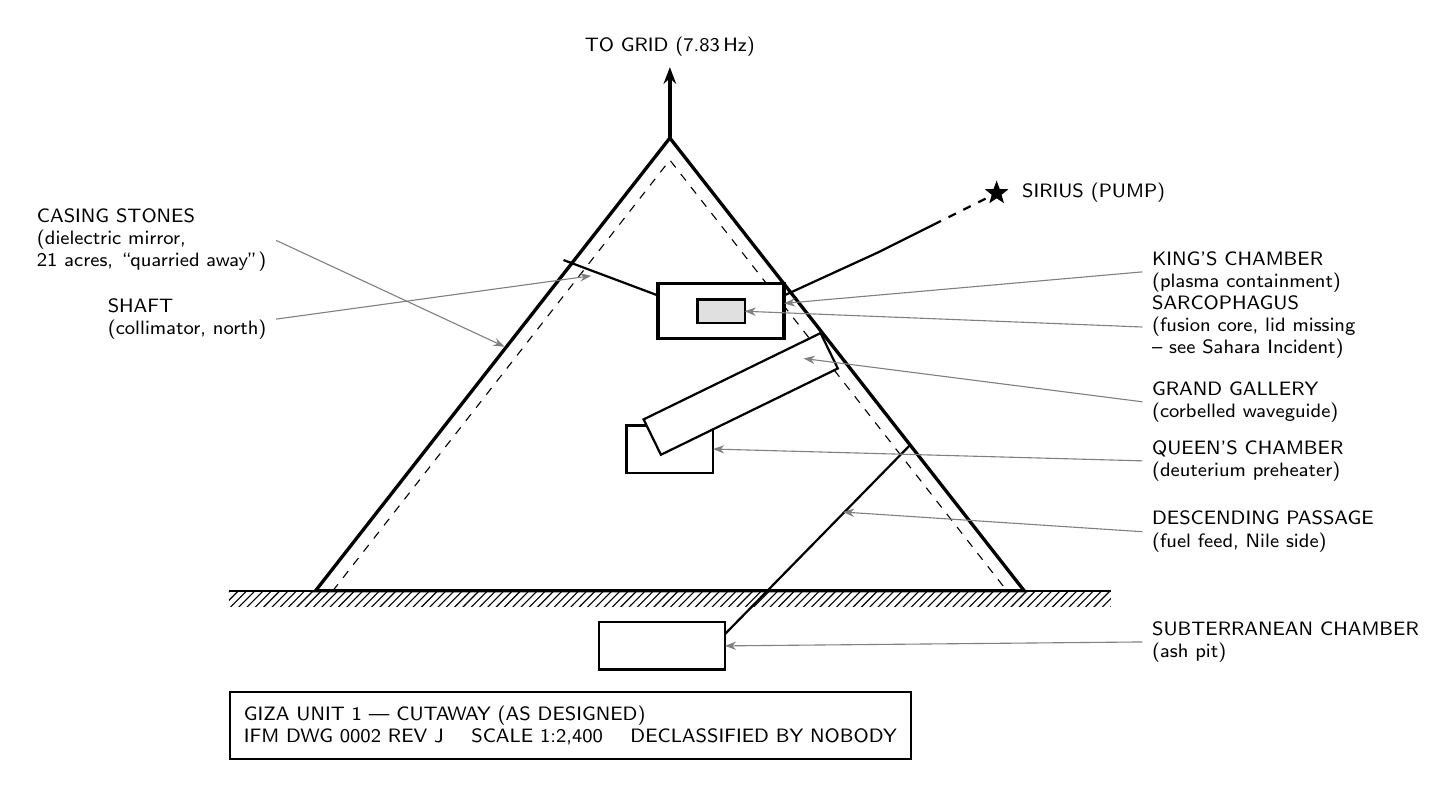
\begin{tikzpicture}[
  lbl/.style={font=\scriptsize\sffamily, align=left},
  pin/.style={-{Stealth[length=4pt]}, gray, thin},
  comp/.style={draw, thick, fill=white}
]
  % ground
  \fill[pattern=north east lines] (-5.6,-1.35) rectangle (5.6,-1.15);
  \draw[thick] (-5.6,-1.15) -- (5.6,-1.15);

  % pyramid shell
  \draw[very thick] (-4.5,-1.15) -- (0,4.6) -- (4.5,-1.15) -- cycle;
  \draw[dashed] (-4.28,-1.15) -- (0,4.32) -- (4.28,-1.15) -- cycle; % casing (missing)

  % subterranean chamber (ash pit)
  \draw[comp] (-0.9,-2.15) rectangle (0.7,-1.55);
  % descending passage
  \draw[thick] (3.05,0.7) -- (0.7,-1.7);

  % queen's chamber (preheater)
  \draw[comp] (-0.55,0.35) rectangle (0.55,0.95);
  % grand gallery (waveguide) — slanted
  \draw[comp, rotate around={26:(0.9,1.35)}] (-0.35,1.1) rectangle (2.15,1.6);
  % king's chamber (containment) + core
  \draw[comp, very thick] (-0.15,2.05) rectangle (1.45,2.75);
  \draw[comp, fill=black!12] (0.35,2.25) rectangle (0.95,2.55);

  % shafts (collimators) + Sirius
  \draw[thick] (1.45,2.6) -- (2.65,3.15) -- (3.35,3.5);
  \draw[thick] (-0.15,2.6) -- (-1.35,3.05);
  \node[star, star points=5, star point ratio=2.4, fill=black,
        minimum size=9pt, inner sep=0pt] (sirius) at (4.15,3.9) {};
  \draw[dashed, thick] (3.35,3.5) -- (sirius);
  \node[lbl, anchor=west] at (4.35,3.9) {SIRIUS (PUMP)};

  % energy out
  \draw[-{Stealth[length=6pt]}, very thick] (0,4.6) -- (0,5.5)
    node[lbl, anchor=south] {TO GRID (7.83\,Hz)};

  % labels, pinned to the right/left
  \node[lbl, anchor=west] (l1) at (6.0,2.9) {KING'S CHAMBER\\(plasma containment)};
  \draw[pin] (l1.west) -- (1.45,2.5);
  \node[lbl, anchor=west] (l2) at (6.0,2.2) {SARCOPHAGUS\\(fusion core, lid missing\\-- see Sahara Incident)};
  \draw[pin] (l2.west) -- (0.95,2.4);
  \node[lbl, anchor=west] (l3) at (6.0,1.25) {GRAND GALLERY\\(corbelled waveguide)};
  \draw[pin] (l3.west) -- (1.7,1.8);
  \node[lbl, anchor=west] (l4) at (6.0,0.5) {QUEEN'S CHAMBER\\(deuterium preheater)};
  \draw[pin] (l4.west) -- (0.55,0.65);
  \node[lbl, anchor=west] (l5) at (6.0,-0.4) {DESCENDING PASSAGE\\(fuel feed, Nile side)};
  \draw[pin] (l5.west) -- (2.2,-0.15);
  \node[lbl, anchor=west] (l6) at (6.0,-1.8) {SUBTERRANEAN CHAMBER\\(ash pit)};
  \draw[pin] (l6.west) -- (0.7,-1.85);
  \node[lbl, anchor=east] (l7) at (-5.0,3.3) {CASING STONES\\(dielectric mirror,\\21 acres, ``quarried away'')};
  \draw[pin] (l7.east) -- (-2.1,1.95);
  \node[lbl, anchor=east] (l8) at (-5.0,2.3) {SHAFT\\(collimator, north)};
  \draw[pin] (l8.east) -- (-1.0,2.85);

  % title block
  \node[draw, thick, lbl, anchor=south west, inner sep=5pt] at (-5.6,-3.3)
    {GIZA UNIT 1 --- CUTAWAY (AS DESIGNED)\\
     IFM DWG 0002 REV J \quad SCALE 1:2{,}400 \quad DECLASSIFIED BY NOBODY};
\end{tikzpicture}
\end{document}
